\documentclass[10pt, a4paper]{article}
\usepackage{graphicx}
%
%%%%%%%%%%%%%%%%%%%%%%%%%%%%%%%%%%%%%%%%%%%%%%%%%%%%%%%%%%%%%%%%%%%%%%%%%%%%
%   document style macros
%%%%%%%%%%%%%%%%%%%%%%%%%%%%%%%%%%%%%%%%%%%%%%%%%%%%%%%%%%%%%%%%%%%%%%%%%%%%
\def\Title#1{\begin{center} {\Large #1 } \end{center}}
\def\Author#1{\begin{center}{ \sc #1} \end{center}}
\def\Address#1{\begin{center}{ \it #1} \end{center}}
\def\andauth{\begin{center}{and} \end{center}}
\def\submit#1{\begin{center}Submitted to {\sl #1} \end{center}}
\newcommand\pubblock{\rightline{\begin{tabular}{l} Proceedings of DIS2022\\ 
         \pubdate  \end{tabular}}}

\newenvironment{Abstract}{\begin{quotation} \begin{center} 
             \large ABSTRACT \end{center}\bigskip 
      \begin{large}}{\end{large}\end{quotation}}

\newenvironment{Presented}{\begin{quotation} \begin{center} 
             PRESENTED AT\end{center}\bigskip 
      \begin{center}\begin{large}}{\end{large}\end{center} \end{quotation}}

\def\Acknowledgements{\bigskip  \bigskip \begin{center} \begin{large}
      \bf ACKNOWLEDGEMENTS \end{large}\end{center}}

%%%%%%%%%%%%%%%%%%%%%%%%%%%%%%%%%%%%%%%%%%%%%%%%%%%%%%%%%%%%%%%%%%%%%%%%%%%% 
%  personal abbreviations and macros
%    the following package contains macros used in this document:
%%%%%%%%%%%%%%%%%%%%%%%%%%%%%%%%%%%%%%%%%%%%%%%%%%%%%%%%%%%%%%%%%%%%%%%%%%%

\textwidth=6.5in
\textheight=8.75in
\hoffset=-0.85in
\voffset=-0.6in


% include packages you will need
\usepackage[utf8]{inputenc}
\usepackage{color}
\usepackage{lineno}
\usepackage{hyperref}
\usepackage[style=phys,%
	biblabel=brackets,%
	chaptertitle=false,pageranges=false,%
	maxnames=4,sorting=none]{biblatex}
\usepackage{amsmath,amsthm,amssymb}
\usepackage{graphicx}
\usepackage{physics}
\usepackage{subcaption}
\usepackage{tikz}
\usepackage{siunitx}
\usepackage{url}
\usepackage[obeyFinal]{todonotes}

\graphicspath{{images/}}
\addbibresource{references.bib}
%%%%%%%%%%%%%%%%%%%%%%%%%%%%%%%%%%%%%%%%%%%%%%%%%%%%%%%%%%%%%%%%%%%%
% basic data for the eprint:
%%%%%%%%%%%%%%%%%%%%%%%%%%%%%%%%%%%%%%%%%%%%%%%%%%%%%%%%%%%%%%%%%%%%


\newcommand\pubdate{\today}

%%  Affiliation
\def\affiliation{
On behalf of SeaQuest Collaboration, \\
Department of Physics, University of Illinois Urbana-Champaign, \\Urbana, Illinois 61801, USA}

%% Acknowledge the support
\def\support{\footnote{Work supported by NSF-2111046}}


\newcommand{\conference}{DIS2022: XXIX International Workshop on Deep-Inelastic Scattering and Related Subjects\\
Santiago de Compostela, Spain\\
May 2-6 2022}

\begin{document}
\large
\begin{titlepage}
	\pubblock


	\vfill
	\Title{Measurement of Charmonium Production in $p + p$ and $p + d$ Interaction in the Fermilab SeaQuest Experiment}
	\vfill

	\Author{Ching Him Leung \support}
	\Address{\affiliation}
	\vfill

	\begin{Abstract}
		SeaQuest has measured dimuon events from the interaction of \SI{120}{\GeV} proton
		beam on liquid hydrogen and deuterium targets with dimuon mass between \num{2}
		and \SI{8}{\GeV}. These dimuon events contain both the Drell-Yan process and the
		charmonium ($J/\psi$ and $\psi^\prime$) production. Unlike the Drell-Yan process
		which probes the antiquark distributions in the nucleons, the charmonium production
		is sensitive to both quark and gluon distributions. SeaQuest has extracted the
		$(p+d)/(p+p)$ cross section ratios as well as the differential cross sections for
		charmonium production in the kinematic region of $0.4 < x_F < 0.9$. The $(p+d)/(p+p)$
		cross section ratios for charmonium production are found to be significantly different
		from that of the Drell-Yan process. The measured differential cross sections for
		charmonium production are compared with theoretical model calculations.
	\end{Abstract}

	\vfill

	\begin{Presented}
		\conference
	\end{Presented}
	\vfill
\end{titlepage}

\setcounter{footnote}{0}
\normalsize


\section{Introduction}
\label{sec:intro}
The SeaQuest experiment at Fermilab was designed to measure high-mass dimuons
produced in the interaction of \SI{120}{\GeV} proton beam with various targets.
Dimuons originating from the Drell-Yan process \cite{drell1970} as well as the
decay of quarkonium states were collected simultaneously. Results from SeaQuest
on the $(p+d)/(p+p)$ Drell-Yan cross section ratios, which are sensitive to
the flavor asymmetry of $\bar{d}/\bar{u}$ in the proton, were reported recently
\cite{dove2021}.

\todo[inline]{$J/\psi$ production}
Unlike the Drell-Yan process which primarily involves the annihilation of quark
and antiquark pair via electromagnetic interaction, charmonium production proceeds
via strong interaction containing contributions from both quark-antiquark
annihilation and gluon-gluon fusion processes.

While proton-induced charmonium production is expected to be dominated by gluon-gluon
fusion process \cite{vogt1999}, some contributions form the quark-antiquark
annihilation process is also expected. The relative importance of these two
processes is expected to depends on the energy of the colliding hadron as well
as the Feynman-$x$ ($x_F$) of the charmonium \cite{peng1995} as illustrated in
Fig.~\ref{fig:cem_comp}.
\begin{figure}[htbp!]
	\centering
	\begin{subfigure}{0.45\linewidth}
		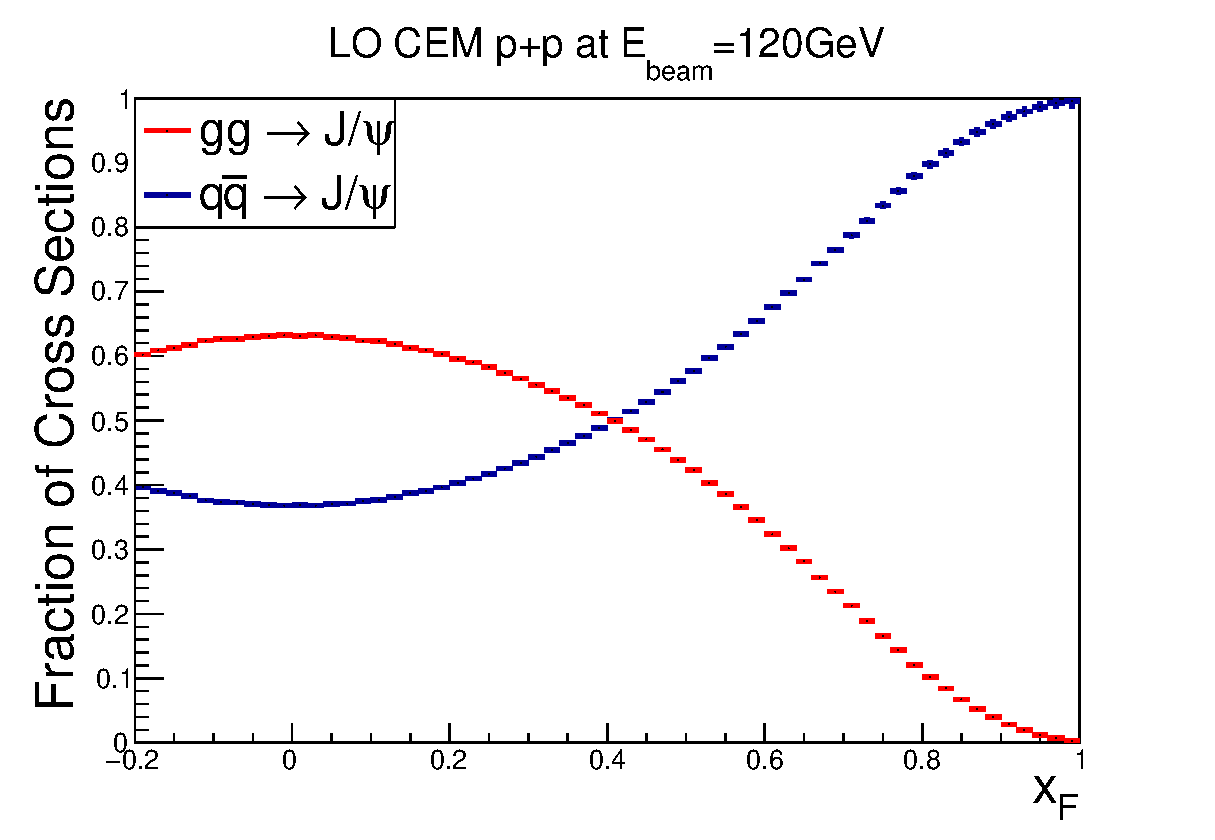
\includegraphics[width=0.9\linewidth]{E906_contribution_LO}
		\caption{}
		\label{subfig:cem_e906}
	\end{subfigure}
	\begin{subfigure}{0.45\linewidth}
		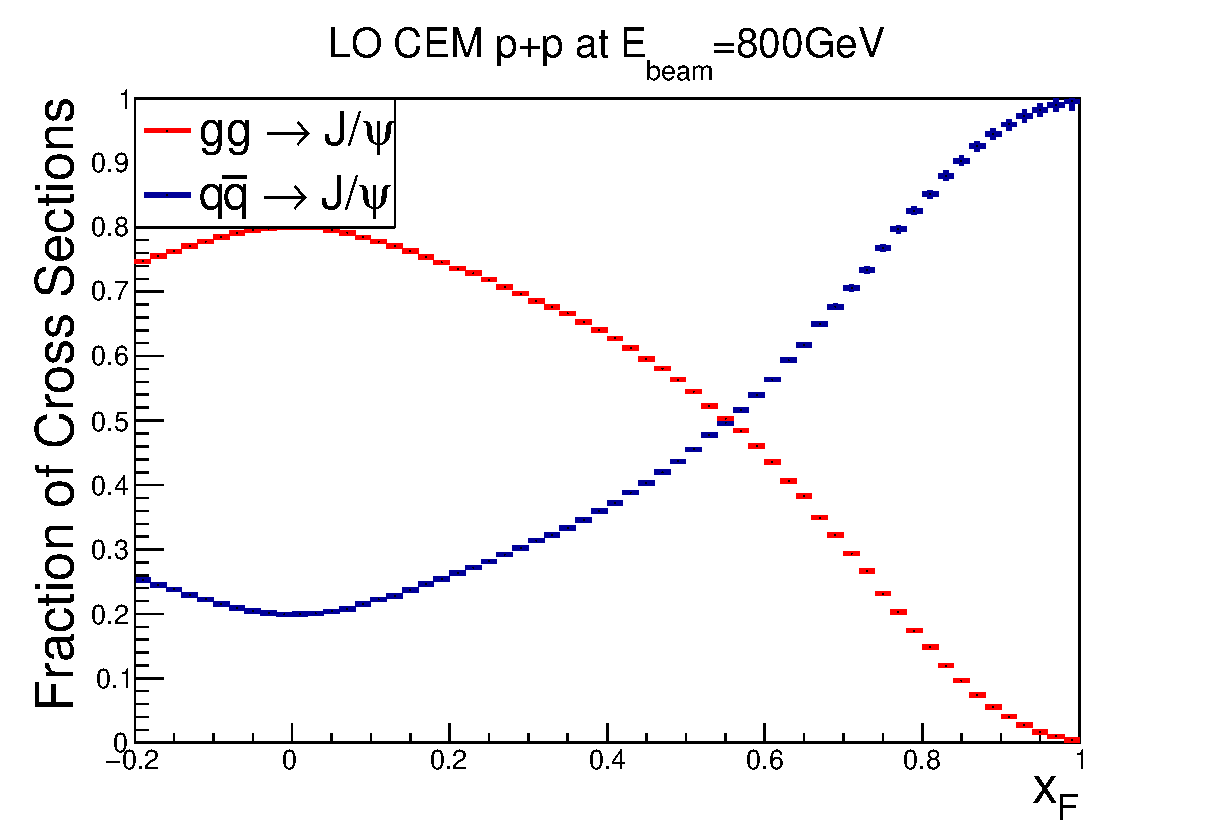
\includegraphics[width=0.9\linewidth]{E866_contribution_LO}
		\caption{}
		\label{subfig:cem_e866}
	\end{subfigure}
	\caption{The relative importance of quark-antiquark annihilation
		and gluon-gluon fusion processes calculated at E906 energy (\subref{subfig:cem_e906})
		and E866 energy (\subref{subfig:cem_e866}) using CEM framework \cite{mangano1993}.}
	\label{fig:cem_comp}
\end{figure}



\section{E906/SeaQuest Experiment}
\label{sec:e906}
SeaQuest is a fixed-target experiment utilizing the \SI{120}{\GeV} proton beam
from the Fermilab Main Injector. Details of the SeaQuest spectrometer can be
found in Ref.~\cite{aidala2019}. The target system consists of seven
interchangeable targets, including a flask with liquid hydrogen, a flask with
liquid deuterium,an empty flask (vacuum), solid carbon, iron, and tungsten
targets as well as a space with no target (air). The targets are interchanged
periodically to reduce systematic uncertainties in the measured cross section
ratios for different targets.

The spectrometer consists of two magnets and four tracking stations. FMag,
placed \SI{104}{\cm} downstream the target, is a \SI{5}{\m} solid iron magnet
that acts as the beam dump as well as a focusing magnet. It is then followed by
the first tracking stations. Stations 1, 2 and 3 each consists of plastic
scintillator hodoscopes and drift chambers. An open air dipole magnet (KMag) is
placed between station 1 and station 2. The vertical magnetic field from both
magnets bends the muons horizontally, allowing the measurement of the momentum
of the muons. Downstream of station 3, there is a 1 m iron wall acting as a
hadron absorber. Station 4 is located behind the hadron absorber and acts as a
muon identifier. Station 4 consists of a hodoscope array and 4 layers of
proportional tube planes. Tracks that pass through the hadron absorber and
produce hits on station 4 are assumed to be from muons.

\section{Extraction of \texorpdfstring{$J/\psi$}{J/psi} cross section}
\label{sec:result}

The $J/\psi$ yield is obtained by studying the mass distribution as shown in
Fig.~\ref{fig:mass}. The mass distribution is fitted by taking into account
several contributions. First, the mass spectrum from the data collected 
with the empty target flask, properly normalized by the integrated beam 
intensity, is shown as the black dash-dot-doted curve. 
\todo{describe the MC and the fitting procedure}

\begin{figure}[htbp!]
	\centering
	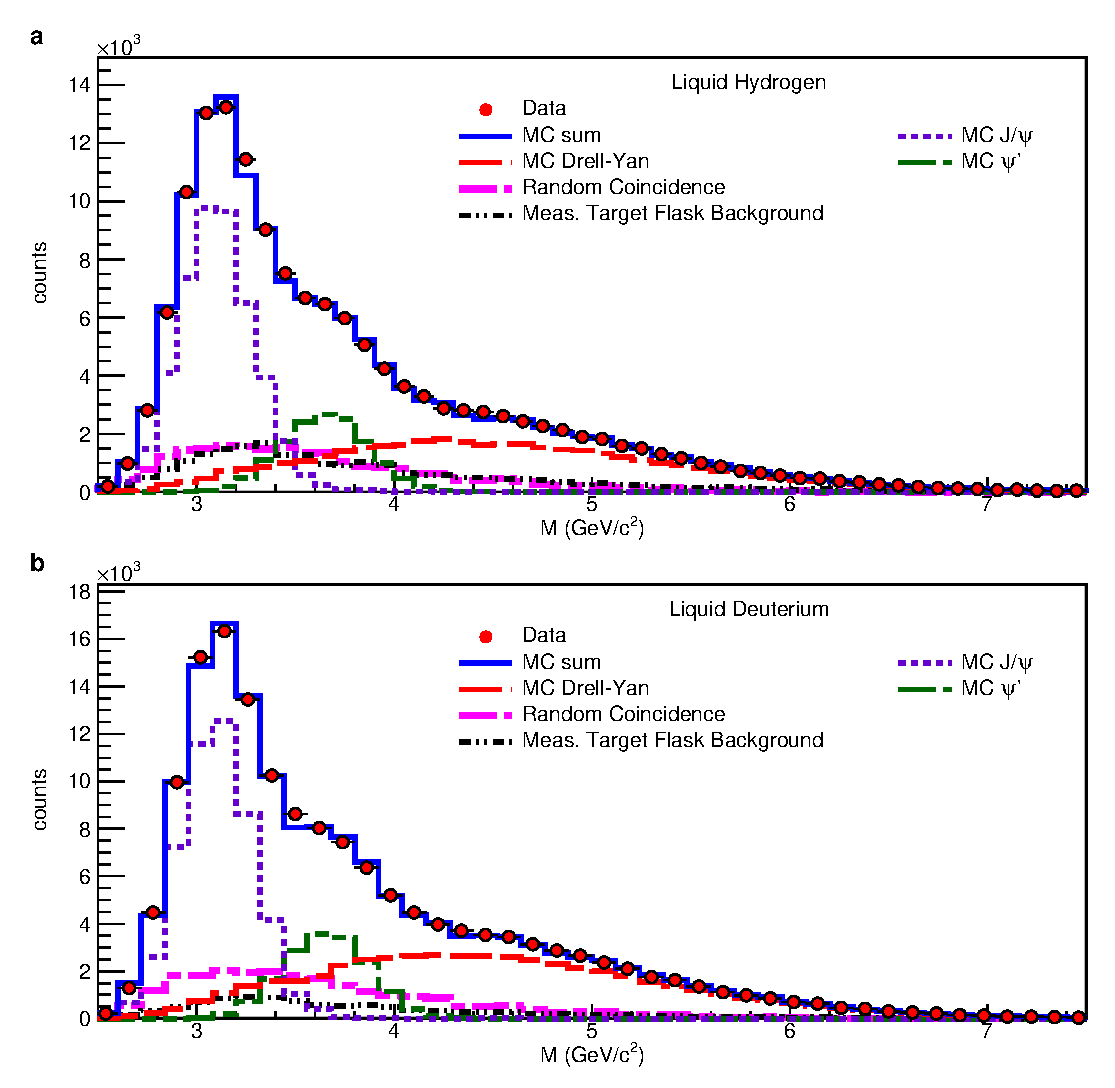
\includegraphics[width=0.7\linewidth]{extFig3}
	\caption{The mass distribution of hydrogen target data (top panel) and
		deuterium target data (bottom panel)\cite{dove2021}\todo[inline]{describe the different color}}
	\label{fig:mass}
\end{figure}

After the number of $J/\psi$ events is extracted from the mass distributions,
the $p+d$ and $p+p$ cross sections can be calculated. And the result is shown in
Fig.\ref{fig:abs_cs_NRQCD}.
\todo{describe the cross section calculation and systematic}
\begin{figure}[htbp!]
	\centering
	\begin{subfigure}{0.45\linewidth}
		\includegraphics[width=0.9\linewidth]{jpsi_xF_LH2}
	\end{subfigure}
	\begin{subfigure}{0.45\linewidth}
		\includegraphics[width=0.9\linewidth]{jpsi_xF_LD2}
	\end{subfigure}
	\caption{The preliminary result on the extracted $J/\psi$ cross section for
		proton on hydrogen (left) and proton on deuterium (right). The result is
		also compared with NRQCD predictions.}
		\label{fig:abs_cs_NRQCD}
\end{figure}
The preliminary is in good agreement with the NRQCD calculation.


\begin{figure}[htbp!]
	\centering
	\begin{subfigure}{0.45\linewidth}
		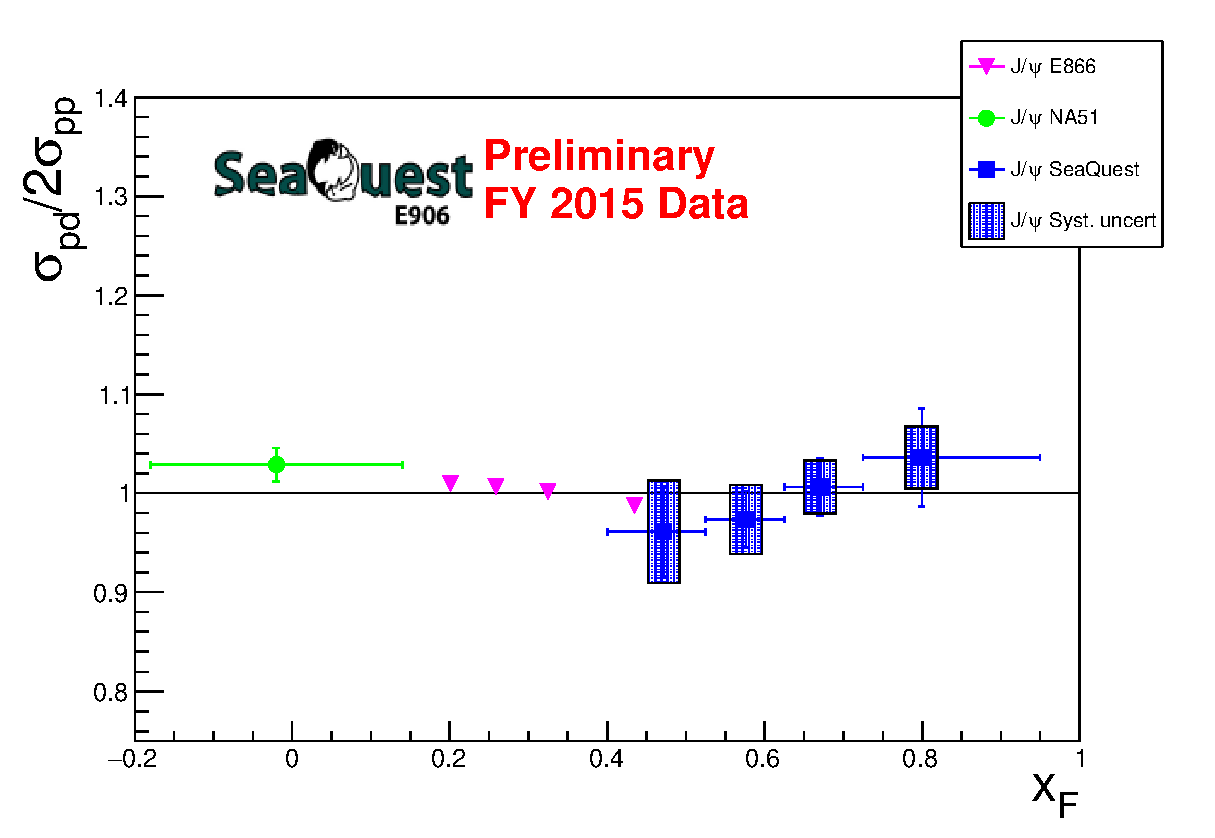
\includegraphics[width=0.9\linewidth]{jPsi_all_noTheory_v2}
	\end{subfigure}
	\begin{subfigure}{0.45\linewidth}
		\includegraphics[width=0.9\linewidth]{jPsi_csr_x2_nature_NRQCD_CEM}
	\end{subfigure}
	\caption{The preliminary result on the extracted $J/\psi$ $(p+d)/2(p+p)$
		cross section ratio as a function of $x_F$ (left) and $x_t$ (right).
		The extracted ratio is also compared with previous measurements by NA51
		\cite{abreu1998} and E866 \cite{peng2003} (left), as well as the Drell-Yan
		cross section ration reported by SeaQuest\cite{dove2021} (right).}
		\label{fig:csr}
\end{figure}
The preliminary $J/\psi$ $(p+d)/2(p+p)$ cross section ratio is shown in
Fig.~\ref{fig:csr}. The preliminary result is consistent with unity within
uncertainty. The difference between the $J/\psi$ and Drell-Yan ratios are
reflecting the different mechanism in the different processes.
\todo{cross section ratios}


\section{Conclusions}


\printbibliography[heading=bibintoc,title={References}]
\listoftodos
\end{document}

